\chapter{Reference Coverage and Granularity}
\label{chp:covgran}

This chapter is based on the following publications.
\begin{infobox-pub}
\fullcite{Saier2022ULITE}
\end{infobox-pub}

\begin{infobox-pub}
\fullcite{Saier2023unarXive}
\end{infobox-pub}

The work in this chapter addresses the following research task.

\begin{rtlist}
    \item[\rtmark{2}:] \textit{Citation Network Completeness} - develop a method to link literature references, that is able to link more references than are linked in existing data sets, while not compromising on link correctness or processing efficiency.
\end{rtlist}

\section{Overview}
In this chapter, we introduce improvements for our corpus creation methodology in two areas.
First, we present in Section~\ref{sec:covgran-blocking} a blocking and matching method applied on the set of references in a corpus. With this, matched references as well as bibliographic couplings can significantly be increased. % Furthermore, it removes the reliance of a ...
Second, we present in Section~\ref{sec:covgran-ux22} an improved conversion method for \LaTeX\ source files, and with it an update of the \emph{unarXive} corpus. The improved corpus creation method enables fine-granularly structured document representations, and achieves a new state-of-the-art reference matching success rate.\footnote{After the publication of our initial corpus creation methodology in \cite{Saier2020} (see Chapter~\ref{chp:corpus}), the now widely used corpus S2ORC~\cite{Lo2020} adapted our document conversion methodology for the \LaTeX\ subset of their data set. While they do not achieve a reference matching success rate as high as ours, they made advances regarding the structured document representation. With the work presented in this chapter, we follow and improve upon their example, establishing a fine-granular structured document representation for the \emph{unarXive} corpus.}

At the end of the chapter, in Section~\ref{sec:covgran-assessment}, we assess the achievement of the research task, as well as the contributions made in terms of the overarching research goal of enabling higher-quality scholarly data.

% \begin{abstract}
% Analyses and applications based on bibliographic references are of ever increasing importance. However, reference linking methods described in the literature are only able to link around half of the references in papers. To improve the quality of reference linking in large scholarly data sets, we propose a blocking-based reference linking approach that utilizes a rich set of reference fields (title, author, journal, year, etc.) and is independent of a target collection of paper records to be linked to. We evaluate our approach on a corpus of 300,000 references. Relative to the original data, we achieve a 90\% increase in papers linked through references, a five-fold increase in bibliographic coupling, and a nine-fold increase in in-text citations covered. The newly established links are of high quality (85\% $\text{F}_1$ score). We conclude that our proposed approach demonstrates a way towards better quality scholarly data.
% \end{abstract}

% \section{A Blocking-Based Approach to Enhance Large-Scale Reference Linking}
\section{Reference Linking by Inter-Reference Blocking}\label{sec:covgran-blocking}

\subsection{Introduction}
% % Motivation
Scholarly data is becoming increasingly important and with it its quality and coverage. Connections between publications in the form of literature references are of particular importance, as they are used as a basis for various analyses, decision making, and applications. Some examples are research output quantification~\cite{Hirsch2005}, trend detection~\cite{Chen2006}, summarization~\cite{Elkiss2008}, and recommendation~\cite{Ma2020,Faerber2020a}.

% Problem
%However, in current data sets providing interlinked publications, only around half of the references contained in the original papers are linked\footnote{We use ``link[ing/ed] references'' w.r.t. to connections to cited papers rather than in-text citation markers.} to the cited publications~\cite{Lo2020,Saier2020}. This lack in coverage is especially affecting references to non-English publications~\cite{Saier2021}, which are in general underrepresented in scholarly data~\cite{Vera-Baceta2019,Liu2019,Moed2018,Moskaleva2019} along with publications in the humanities~\cite{Colavizza2019,Kellsey2004}.
However, reference linking methods\footnote{In the following, we use ``link[ing/ed] references'' to refer to connections to cited papers rather than in-text citation markers.} described in the literature are only able to link around half of the references contained in the original papers to the cited publications~\cite{Lo2020,Saier2020}. This lack in coverage is especially affecting references to non-English publications~\cite{Saier2021}, which are in general underrepresented in scholarly data~\cite{Vera-Baceta2019,Liu2019,Moed2018,Moskaleva2019} along with publications in the humanities~\cite{Colavizza2019,Kellsey2004}.

We see the reason for this lack in linked references in two key shortcomings of current methods.
First, references are linked using simple string similarity measures that are often relying \emph{only} on publications' title and author information (which is not always contained in references; see Figure~\ref{fig:hardmatch}). %Note: maybe add sth. along the lines of “relying on title (and mby authors) is deemed sufficient”
Second, references are exclusively linked to a target collection of paper records---usually a large metadata set like DBLP\refurl{https://dblp.org/}{2023-11-10} or OpenAlex,\refurl{https://openalex.org/}{2023-11-10} or a set of IDs like DOIs or PMIDs. This means references to literature which is not contained in the target collection, as well as to non-source items~\cite{Chi2014}, cannot be linked (see ``?'' markers in Figure~\ref{fig:approach}).

\begin{figure}[tb]
  \centering
  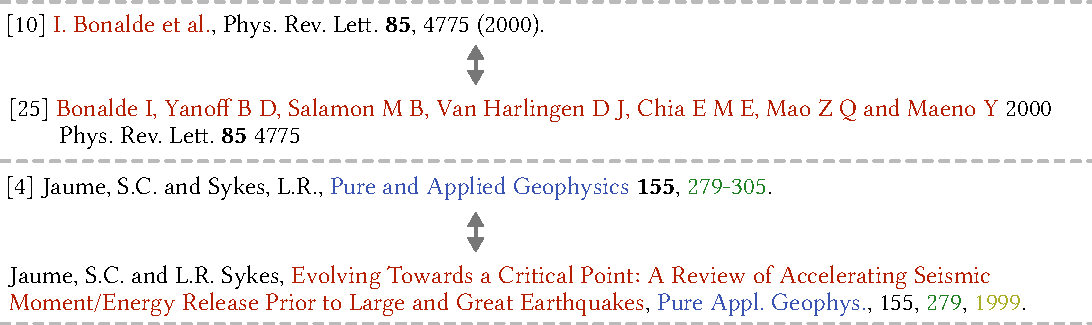
\includegraphics[width=\linewidth]{figures/ref_covgran/hardmatch_examples.pdf}
  \caption[Examples of challenging reference pairs from our evaluation that where successfully matched]{Examples of challenging reference pairs from our evaluation that where successfully matched. \textbf{Top:} references from \texttt{arXiv:cond-mat/0503317} (no title, first author only) and \texttt{arXiv:cond-mat/0104493} (no title, all authors). \textbf{Bottom:} references from \texttt{arXiv:cond-mat/0104341} (no title, full venue, page rage, no year) and \texttt{arXiv:physics/0504218} (with title, venue abbreviation, start page only, with year).}
  \label{fig:hardmatch}
\end{figure}

\begin{figure}[tb]
  \centering
  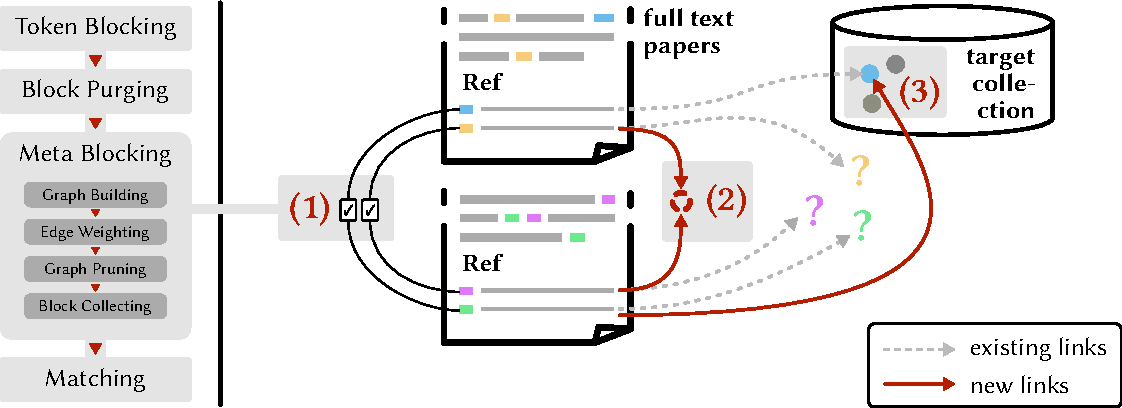
\includegraphics[width=\linewidth]{figures/ref_covgran/approach_withblocking_10pvar.pdf}
  \caption[Schematic depiction of the use case]{Schematic depiction of the use case. A corpus of full-text papers, where some references are already linked to a target collection (blue), and some are not (orange, pink, green). At \textbf{(1)} we apply our blocking and matching approach to identify all references that point to the same publication. In doing so, we establish new links in the form of \textbf{(2)} bibliographic coupling and \textbf{(3)} links to the target collection.}
  \label{fig:approach}
\end{figure}

%ER related work
Linking references can be seen as a task of entity resolution~\cite{Christophides2015ERdef}, which is concerned with identifying entities referring to the same object within or between large data sets. Because the task requires a one-to-one comparison between each of the involved entities, it is inherently of quadratic complexity. To make approaches scalable, entities are assigned into groups of likely matching candidates prior to comparison, a technique called blocking~\cite{Papadakis2020survey}.
While blocking-based approaches are used in the domain of scholarly data to, for example, identify duplicate paper records~\cite{Simonini2016blast,Sefid2019,Lo2020} (where information such as abstracts are used) and authors~\cite{FaerberLin2022}, they are not utilized for bibliographic references.

% Our solution
We therefore address both of the aforementioned problems with current reference linking approaches, (1)~the use of simple matching methods based on title and authors, as well as (2)~the reliance on a target collection of paper records, by proposing (1)~the use of a blocking and matching process utilizing seven reference fields (title, author, journal, year, etc.) that (2)~operates \emph{within} the set of bibliographic references of a corpus, and is thereby \emph{independent} of a target collection of papers (see marker ``(1)'' in Figure~\ref{fig:approach}).

We showcase the feasibility and benefits of our approach, implementing a pre-processing, blocking, and matching pipeline and evaluating it on a corpus containing 300,000 references.
We show that relative to the original data, our approach gives us a \textbf{90\% increase} in papers linked to the target collection, a \textbf{five-fold increase} in bibliographically coupled~\cite{Boyack2010} papers (see marker ``(2)'' in Figure~\ref{fig:approach}), and a \textbf{nine-fold increase} in in-text citation markers covered.\footnote{With the ``coverage'' of in-text citation markers we refer to markers associated with linked references, relative to markers belonging to unlinked references.} The new links are furthermore of high quality (85\% $\text{F}_1$ score). This paves the way towards higher quality scholarly data, especially regarding the coverage of so far underrepresented literature and non-source items.

In summary, we make the following contributions.

\begin{itemize}
    \item We propose a blocking-based approach for matching bibliographic references that is independent of a target collection of paper records.
    \item We perform a large-scale evaluation showing that our approach results in a manifold increase in high-quality reference links.
    \item We make our data and code publicly available.\refurl{https://github.com/IllDepence/ulite2022}{2023-11-10}
\end{itemize}

\subsection{Related Work}
Blocking-based approaches have been used in the domain of scholarly data, though to the best of our knowledge not for bibliographic references. We therefore report on (1) exemplary uses of blocking in the scholarly domain for entities other than references, and (2) approaches to linking bibliographic references using methods other than blocking.

Simonini et al.~\cite{Simonini2016blast} develop BLAST (Blocking with Loosely-Aware Schema Techniques) which adapts Locality-Sensitive Hashing. Among data sets from other domains, they also evaluate their approach for the task of linking 2,600 DBLP paper records to the ACM\refurl{https://dl.acm.org/}{2023-11-10} and Google Scholar.\refurl{https://scholar.google.com/}{2023-11-10} 
Sefid~\cite{Sefid2019} proposes several models to match paper records utilizing the papers' title, header, and citation information. The models are evaluated in three scenarios matching 1,000 paper records from CiteSeer$^x$~\cite{CiteSeerX2019} to IEEE, DBLP, and Web of Science.
Lastly, Färber et al.~\cite{FaerberLin2022} detect duplicates among 243 million author records in the Microsoft Academic Knowledge Graph~\cite{MAKG} and evaluate their approach using ORCiD IDs.

%                        GROBID | LaTeX
% Bibliography entries   27.6M  | 21.9M*
% Linked bib. entries    19.3M  |  6.8M*
%
% *The lower number of linked bibliography entries in latex parses is due to large numbers of papers (mostly in the field of physics) for which the bibliography entries are formatted without paper titles. Our linking algorithm strongly depends on titles and fails to link these entries.
Lo et al.~\cite{Lo2020} introduced the data set S2ORC, which contains 9.6 million open access papers and has recently seen extensive use in area of scholarly document processing. The authors link references to papers within their data set using a heuristic similarity measure based on n-grams and the Jaccard similarity, which only uses the paper title. Using this method, 26 million out of 50 million references  (52\%) are successfully linked. The authors report that the low number is \textit{``due to large numbers of papers (mostly in the field of physics) for which the bibliography entries are formatted without paper titles.''} Saier et al.~\cite{Saier2020} introduce unarXive, a data set created from papers' \LaTeX\ sources containing over 1 million publications. Bibliographic references in the data set are linked to the Microsoft Academic Graph~\cite{Sinha2015,Wang2019}. The linking procedure is based on string similarity of papers' titles and author information. With this procedure 17 million out of 40 million references (42\%) are successfully linked.
Lastly, CiteSeer$^x$~\cite{Wu2015,CiteSeerX2019} in another large data set containing paper records. Similar to S2ORC, references are linked to paper records within the data set itself. In the case of CiteSeer$^x$ the linking is performed through a heuristic assignment based on title and author information.  We are not aware of information on the percentage of references that are successfully linked in CiteSeer$^x$.

%ad hoc~\cite{Kokash2022}
%web services often just link to search (lmgtfy)

\subsection{Approach}

Our approach consists of the following three steps: (1) \emph{pre-processing} to convert references into a normalized, structured format, (2) \emph{blocking} to allow us to process large amounts of references, and (3) \emph{matching}. These steps are explained in more detail below.

%Our approach consists of the following three steps: (1)~\emph{pre-processing} to convert references into a normalized, structured format, (2)~\emph{blocking} to allow us to process large amounts of references, and (3)~\emph{matching} to determine references that refer to the same publication. Conceptually the steps operate on the level of (1)~single entities, (2)~blocks (sets of entities or entity pairs), and (3)~entity pairs. Below the steps are explained in more detail.

\paragraph{Pre-processing}
References as they appear in papers are hard to match for several reasons, such as the variety of citation styles, variants of author names, venue abbreviations, sparsity of information, and typing errors~\cite{Christen2012} (see Figure~\ref{fig:hardmatch}). To mitigate these issues, we pre-process references in three steps: first, we apply GROBID's~\cite{Lopez2009} reference string parsing module,\refurl{https://grobid.readthedocs.io/en/latest/Grobid-service/\#apiprocesscitation}{2023-11-10}\textsuperscript{,}\footnote{GROBID was chosen according to the results of~\cite{Tkaczyk2018}.} then we expand journal and conference abbreviations, and lastly all strings are lowercased and Unicode normalized. For the abbreviation expansion we use a mapping for 47.6k journal titles provided by JabRef\refurl{https://github.com/JabRef/abbrv.jabref.org}{2023-11-10} and 2.6k conference titles crawled from various web sources. Following~\cite{Koo2011} we select seven reference fields for the blocking step: title, author, year, volume, journal, booktitle, and pages.

\paragraph{Blocking}
%Blocking is an essential technique in the field of ER~\cite{Papadakis2020survey} used to reduce the number of necessary one-to-one comparisons in or between large data sets. 
%Following~\cite{Papadakis2016}, we build our pipeline with two blocking components, namely  (1)~block building, and (2)~block cleaning. In the subsequent matching step a third component, (3)~comparison cleaning, is applied. As shown in Figure~\ref{fig:approach}, we use token blocking, block purging, and meta-blocking respectively for each of the three steps.
Following~\cite{Papadakis2016}, we build our blocking pipeline from components for (1) block building, (2) block cleaning, and (3) comparison cleaning. As shown in Figure~\ref{fig:approach}, we use token blocking, block purging, and meta-blocking respectively for each of the steps.

\emph{Token blocking} is chosen for the block building step because it is schema-agnostic and therefore robust against the varying level of information contained in or missing from bibliographic references. In this step, references are assigned to blocks based on all tokens (i.e., words) contained in the identified and normalized reference fields. As a result, references at this point are associated with multiple blocks, which leads to a high level of redundancy.

\emph{Block purging}~\cite{Papadakis2011blockpurging} removes oversized blocks based on a comparison cardinality metric, which we determine heuristically and set it to 0.01. Intuitively, the removed blocks originate from common tokens, meaning that matched reference strings within them are highly likely to also share smaller blocks. Purging therefore reduces the number of overall comparisons with minimal effect on the final result quality.

\emph{Meta-blocking}~\cite{Papadakis2014}, our comparison cleaning step, reduces unnecessary comparisons within blocks by generating a weighted graph of entities (references in our case) based on their shared blocks, removing edges based on a pruning scheme, and lastly creating a new block collection based on the reduced graph. For both the weighting and the pruning of edges several schemes exist. In Section~\ref{sec:eval} we describe how we determined the most suitable combination of schemes for our use case. Here, we briefly mention the schemes involved. Available graph weighting schemes include the Common Blocks Scheme (CBS), the Enhanced Common Blocks Scheme (ECBS), the Aggregate Reciprocal Comparisons Scheme (ARCS), and the Jaccard Scheme (JS). For graph pruning, we consider Cardinality Node Pruning (CNP), which relies on cardinality to select the top edges for each node, as well as Weight Edge Pruning (WEP), which removes edges based on their assigned weight.

% \emph{Meta-blocking}~\cite{Papadakis2014}, our comparison cleaning step, reduces unnecessary comparisons within blocks and consists of four sub-steps: graph building, edge weighting, graph pruning, and block collecting.

% In the \emph{graph building} step, the block collection is transformed in a blocking graph, where an entity (i.e., reference string) is represented as a node, and the co-occurrence of two entities in a common block is conveyed by an edge connecting them. Since a new edge is only created for a pair of entities that hasn’t appear yet. If a pair of entities share more than one block, they will only be connected by one edge and will not appear repeatedly in the blocking graph. 

% The information conveyed through the number of blocks shared by a pair of entities is entailed in the weight of the edge between the pair, which is determined in the \emph{edge weighting} step relying on a weighting scheme. There are five weighting schemes available: (1)	Aggregate Reciprocal Comparisons Scheme(ARCS), (2)	Common Blocks Scheme(CBS), (3) Enhanced Common Blocks Scheme(ECBS), (4)	Jaccard Scheme(JS), and (5)	Enhanced Jaccard Scheme(EJS).

% In the next step, \emph{graph pruning} depends on a pruning scheme to prune the weighted blocking graph. There are four pruning schemes available: (1)    Weight Edge Pruning(WEP), examines all the edges in the blocking graph and remains those, whose weight reaches a minimum edge weight, (2)    Cardinality Edge Pruning(CEP), only those top edges with the highest weight in the blocking graph are remained according to a cardinality threshold, (3)    Weight Node Pruning(WNP), set a local weight threshold for each node to discard edges that linked to the node, and (4)    Cardinality Node Pruning(CNP), relies on a cardinality threshold to select the top edges for each node from all the edges that linked to the node.

% As the last step of blocking, \emph{block collecting} creates a new block collection with all remaining reference strings based on the pruned blocking graph.

\paragraph{Matching}

To determine which references within a block refer to the same publications, we utilize a weighted average of Jaccard similarities across our seven reference fields. Based on~\cite{Foufoulas2017} as well as preliminary experiments, we set the weights for title, author, journal, booktitle, year, volume, and pages to $8$, $6$, $5$, $5$, $3$, $3$, and $2$ respectively, and set the threshold for a match to $0.405$.

% \paragraph{Matching}
% After blocking, whether reference strings within the same blocks match the same document or not should be determined. Among various similarity measures~\cite{Christen2012}, token-based metrics are better suited to comparing long strings involving multiple tokens. We apply Jaccard similarity metric for computing similarity between reference strings,which measures the percentage of common tokens shared by both strings and is calculated as the common tokens within both strings divided by the number of all distinct tokens in both strings.  

% Based on~\cite{Foufoulas2017} and preliminary experiments, we assign different weight to different metadata fields, and compute the similarity for each metadata field separately to avoid mismatch when the same token appears in different fields and at the same time, to consider the different importance of different metadata fields. 
% Taking the coverage of metadata fields into account, we calculate the value of $SumSim$ by adding the weighted Jaccard similarity value of all the selected fields together.
% \begin{equation}
%   \begin{aligned}
%   {SumSim}=8\times{sim}_{Jaccard}(title)+6\times{sim}_{Jaccard}(author)+5\times{sim}_{Jaccard}(journal)\\
%   +5\times{sim}_{Jaccard}(booktitle)+3\times{sim}_{Jaccard}(year)\\
%   +3\times{sim}_{Jaccard}(volume)+2\times{sim}_{Jaccard}(pages)
%   \end{aligned}
% \end{equation}

% In order to ensure that the value of final similarity falls in the interval [0,1], the final similarity between a pair of reference strings $p_j$ and $p_k$ is defined as the value of $SumSim(p_{j},p_{k})$ divided by the maximum value of the function $SumSim$ (i.e., $MaxVal$ below):

% \begin{equation}
%   {sim}(p_{j},p_{k})= \dfrac{{SumSim}(p_{j},p_{k})}{MaxVal}
% \end{equation}

% After calculating the similarity between all pairs in the resulting block collection, if the similarity value reaches the matching threshold (set to 0.405 based on preliminary experiments), the pair is thus recognized as a match. Otherwise, they are decided as non-match. 

\subsection{Evaluation}\label{sec:eval}

We use a large corpus of scholarly publications to perform two types of evaluations. (1)~A large-scale evaluation utilizing the corpus' existing reference links as ground truth, and (2)~a manual evaluation to also assess the correctness of newly created reference links. In the following, we describe the data used, evaluations performed, and results obtained.

\paragraph{Data}
For our evaluation we use the data set unarXive~\cite{Saier2020}. We chose this data set over similar data sets such as S2ORC~\cite{Lo2020}, because it not only contains paper's full-text with annotated in-text citation markers, but also a dedicated database of all raw references in plain text. From unarXive we sample the 300,000 most recent references to conduct our evaluation. The 300,000 references originate from 9,917 papers from the disciplines of physics (7,347), mathematics (1,686), computer science (789), and other STEM fields (95). The publications cited through the references cover publication years from 1743 up to 2020. Four examples of references used in the evaluation are shown in Figure~\ref{fig:hardmatch}.

% \paragraph{Result}
% As a first step, token blocking generates 116,826 blocks in total with a minimum size of 2 and a maximum size of 70,372. 
% % mention through a heuristic attempt of different purging thresholds?
% In the blocking purging step, the purging threshold is calculated as 0.01. In consequence, the maximum block size is 22 and the number of comparisons after block purging is 16,585,773.
% Since meta-blocking involves five weighting schemes as well as four pruning algorithms, there exists 20 different combinations in total. 



\paragraph{Large-Scale Evaluation}

%Common Blocks Scheme(CBS)
%Enhanced Common Blocks Scheme(ECBS)
%Aggregate Reciprocal Comparisons Scheme(ARCS)
%Jaccard Scheme(JS)
%  (Enhanced Jaccard Scheme(EJS))

%Cardinality Node Pruning (CNP)
%Weight Edge Pruning (WEP)
%  (Cardinality Edge Pruning (CEP))
%  (Weight Node Pruning (WNP))

%Pair Completeness (PC)
%Pairs Quality (PQ)
%Reduction Ratio (RR)

\begin{table*}
   \caption{Performance of five graph weighting and graph pruning scheme combinations for meta-blocking.}
   \label{tab:evaluation}
   \begin{small}
   \begin{threeparttable}
   \begin{tabular}{ccccccc}
     \toprule
     Weighting scheme & Pruning scheme & \#Comparisons & \#Matches & RR\tnote{1} \ (\%) & PC\tnote{2} \ (\%) & PQ\tnote{3} \ (\%) \\
     \midrule
     CBS\tnote{4} & CNP\tnote{8} & 39,050 & 3,053 & 99.96 & 54.47 & 7.82\\
     ECBS\tnote{5} & CNP & 39,050 & 3,201 & 99.96 & \textbf{57.11} & \textbf{8.20}\\
     ARCS\tnote{6} & CNP & 39,050 & 2,890 & 99.96 & 51.56 & 7.40\\
     ARCS & WEP\tnote{9} & 24,175 & 1,285 & \textbf{99.98} & 22.93 & 5.32\\
     JS\tnote{7} & WEP & 42,919 & 2,272 & 99.96 & 40.54 & 5.29\\
   \bottomrule
 \end{tabular}
    \begin{footnotesize}
    \begin{tablenotes}
      \item[] \textit{Metrics:} \footnotemark[1]Reduction Ratio, \footnotemark[2]Pair Completeness, \footnotemark[3]Pairs Quality
      \item[] \textit{Weighting schemes:} \footnotemark[4]Common Blocks Scheme, \footnotemark[5]Enhanced Common Blocks Scheme, \footnotemark[6]Aggregate Reciprocal Comparisons Scheme, \footnotemark[7]Jaccard Scheme
      \item[] \textit{Pruning schemes:} \footnotemark[8]Cardinality Node Pruning, \footnotemark[9]Weight Edge Pruning
   \end{tablenotes}
   \end{footnotesize}
  \end{threeparttable}
  \end{small}
\end{table*}

Our large-scale evaluation is performed in two steps. First, we determine the most suitable configuration of graph weighting and pruning scheme for our meta-blocking step, then we apply our pipeline to the evaluation corpus and determine the number of additionally linked entities.

To chose a graph weighting and pruning scheme, we use the 13,976 references in our corpus which are are already linked to the target collection as ground truth. Following~\cite{Papadakis2014}, we select five combinations of schemes to evaluate. The combinations are evaluated using the metrics pair completeness (PC), which expresses the ratio of detected matches with respect to all true matches, pair quality (PQ), which estimates the portion of true matches within all executed comparisons in the block collection, and reduction ratio (RR), which measures the number of unnecessary comparisons that are saved through blocking. Table~\ref{tab:evaluation} shows the results of our evaluation. We achieve the best results using ECBS weighting and CNP pruning. Accordingly, we apply our pipeline with this configuration on the full evaluation corpus of 300k references, where our approach performs 496,051 comparisons after blocking and identifies 71,826 matches.

\begin{table*}
   \centering
   \caption{Number of linked papers, references, and in-text citations given in the original corpus and newly created through the application of our approach.}
   \label{tab:newlinks}
   \begin{small}
   \begin{threeparttable}
   \begin{tabular}{rccc}
     \toprule
     \ & \multicolumn{3}{c}{Linked to target collection} \\
     \midrule
     \ & \#Papers & \#Referencecs & \#In-text Citations \\
     Given & 1,590 & 13,975 & 23,707 \\
     New & 1,443 & 2,442 & 7,824 \\
     \midrule
     \ & \multicolumn{3}{c}{Linked through bibliographic coupling} \\
     \midrule
     \ & \#Papers & \#Referencecs & \#In-text Citations \\
     Given & - & - & - \\
     New & 8,895 & 53,940 & 219,630 \\
     \midrule
     \ & \multicolumn{3}{c}{Combined (linked in either way)\tnote{1}} \\
     \midrule
     \ & \#Papers & \#Referencecs & \#In-text Citations \\
     Given & 1,590 & 13,975 & 23,707 \\
     New & 8,931 & 55,197 & 227,454 \\
   \bottomrule
 \end{tabular}
    \begin{footnotesize}
    \begin{tablenotes}
      \item[1] Note that the combined entity counts are not simply the sum of the numbers above, because a single entity can be linked in both ways.
  \end{tablenotes}
   \end{footnotesize}
  \end{threeparttable}
  \end{small}
\end{table*}

%As shown earlier in Figure~\ref{fig:approach}, we can use the matches identified by our pipeline to create two types of new links. First, new links to the target collection (see marker ``(3)'' in Figure~\ref{fig:approach}), and second, links between references created through bibliographic coupling (see marker ``(2)'' in Figure~\ref{fig:approach})
As shown earlier in Figure~\ref{fig:approach}, we can use the matches identified by our pipeline to create two types of new links. First, new links to the target collection, and second, links between references created through bibliographic coupling. New links to the target collection are established whenever a reference with no existing link is matched to a reference with an existing link (see marker ``(3)'' in Figure~\ref{fig:approach}). In cases where neither of the references in a match have an existing link, we create a bibliographic coupling (see marker ``(2)''  in Figure~\ref{fig:approach}).
In Table~\ref{tab:newlinks} we show on the level of papers, references, and in-text citations how many links were already given in our corpus and how many new links we are able to establish. Regarding links to the target collection, we are able to link \emph{1,443 new papers} (90.75\% increase) through \emph{2,442 references} (17.47\% increase), which are connected to \emph{7,824 in-text citation markers} (33.00\% increase). As for bibliographic coupling, we connect \emph{8,895 papers} through \emph{53,940 references} connected to \emph{219,630 in-text citation markers}. Comparing the number of given links to the combined number of new links, we see a 90\% increase in papers linked to the target collection, a five-fold increase in bibliographically coupled papers, and a nine-fold increase in in-text citation markers covered.

% # ## increase
% # (1) citation graph (newly linked to the MAG)
% # - papers:             1,590 + 1,443 -> 90.75% increase
% # - references:         13,975 + 2,442 -> 17.47% increase
% # - in-text markers:    23,707 + 7,824 -> 33.00% increase
% # (2) couplings (not linked to MAG, but linked to each other)
% # - papers:             1,590 vs 8,895 -> 5.59 times of linked
% # - references:         13,975 vs 53,940 -> 3.86 times of linked
% # - in-text markers:    23,707 vs 219,630 -> 9.26 times of linked
% #
% # (3) connected (=resolved or coupled =both of the above)
% # - papers:             1,590 vs 8,931 -> 5.62 times of linked
% # - references:         13,975 vs 55,197 -> 3.95 times of linked
% # - in-text markers:    23,707 vs 227,454 -> 9.59 times of linked 

\paragraph{Manual Evaluation}
To assess the quality of our newly linked references, we take a random sample of 500 reference comparisons from the matching procedure and manually verify if our approach correctly labeled each pair as a match or non-match. This is done by inspecting both original reference strings (prior to pre-processing) and determining whether they refer to the same publication or not. Because in some disciplines such as physics it is common to see references without a title given, this process involves looking up and verifying publications' details online.\footnote{For further details see \refurlinline{https://github.com/IllDepence/ulite2022/tree/master/5_manual_evaluation}{2023-11-10}.} Examples of two reference pairs are shown in Figure~\ref{fig:hardmatch}. Comparing our predicted matches with the manually established ground truth, we measure a precision of 93.20\% and a recall of 79.34\%. Accordingly the $\text{F}_1$ score is 85.71\%.
This shows us that our newly established links are of good quality, suggesting our approach facilitates the creation of more accurate scholarly data and, accordingly, higher quality analyses and downstream applications based scholarly data sets.
%This shows us that most of our newly established links are correct and that the number of missed links is (false negatives) is not very high.\footnote{Note that, due to the nature of our evaluation, the recall value concerns comparisons \emph{within} blocks. This means further missing links for matching references which were not placed together in any block can exist. An evaluation is unfortunately only feasible using comparisons within blocks rather than any random pairs of references in the corpus, because in the latter case the chances are very low that a random sample contains any reference pairs which were considered after blocking.}

\subsection{Discussion and Future Work}
To improve the quality of reference linking in large scholarly data sets, we proposed a blocking-based reference linking approach that is independent of a target collection of paper records. In a large-scale evaluation, we first determined the most suitable meta-blocking scheme for our particular application case. Subsequently applying our approach to a corpus of 300,000 references, we saw a manifold increase in linked papers, references, and in-text citation markers. The newly established links are of high precision and have a high recall, which we confirmed through a manual evaluation on a sample of our results. This demonstrates the benefits and quality of our approach.

Key limitations of the work presented are (1)~the size and discipline coverage of the evaluation corpus, (2)~the usage of a comparatively basic blocking technique, and (3)~the lack of a thorough evaluation of time performance.

In the future we want to address these points by expanding our work through using more advanced blocking methods such as progressive blocking~\cite{Simonini2019,Galhotra2021}, using larger evaluation corpora such as the whole unarXive data set, including data from more diverse disciplines such as the humanities, and evaluating the time performance of our approach.
%Because in our evaluation corpus references are linked to in-text citation markers in the paper full-text, we furthermore plan to explore possible application scenarios using the full-text such as citation context analysis for non-source items.
Because references in our evaluation corpus are linked to in-text citation markers, we furthermore plan to explore application scenarios utilizing the paper full-text. %, such as citation context analysis for non-source items.

% Discussion:
% - Limitations:
%    - not full unarXive corpus
%    - current approach too slow
%    - only evaluated in STEM area
% - Impact:
%    - analyses (more complete citation graph, bibl. coupling of non-source items, ...)
% Future work:
% - More recent blocking/matching approach
% - include target collection into blocking&matching
%   (mby two-step s.t. from b&m in refs a "canonical representation" emerges)
% - whole unarXive corpus
% - other corpora (esp. humanities)

\subsection*{Author Contributions}  % cf. https://casrai.org/credit/
Tarek Saier: Conceptualization, Data curation (support), Formal analysis, Investigation (support), Methodology (support), Software (final evaluation), Visualization, Supervision, Writing -- original draft (lead), Writing -- review \& editing. Meng Luan: Data curation, Formal analysis, Investigation, Methodology, Software, Writing -- original draft (support). Michael F{\"a}rber: Supervision, Writing -- review \& editing.


% \section{unarXive 2022: All arXiv Publications Pre-Processed for NLP, Including Structured Full-Text and Citation Network}
\section{Reference \& Text Granularity - a Corpus Update}\label{sec:covgran-ux22}

% \begin{abstract}
% Large-scale data sets on scholarly publications are the basis for a variety of bibliometric analyses and natural language processing (NLP) applications. Especially data sets derived from publication's \emph{full-text} have recently gained attention.
% While several such data sets already exist, we see key shortcomings in terms of their domain and time coverage, citation network completeness, and representation of full-text content.
% To address these points, we propose a new version of the data set unarXive.
% We base our data processing pipeline and output format on two existing data sets, and improve on each of them. Our resulting data set comprises 1.9 M publications spanning multiple disciplines and 32 years. It furthermore has a more complete citation network than its predecessors and retains a richer representation of document structure as well as non-textual publication content such as mathematical notation. In addition to the data set, we provide ready-to-use training/test data for citation recommendation and IMRaD classification. All data and source code is publicly available at \refurlinline{https://github.com/IllDepence/unarXive}{2023-111-10}.
% \end{abstract}

\subsection{Introduction}
% - - - - - Why are full-text scholarly data sets relevant? - - - - -

% paper motivation: since the release of unarXive, and S2ORC shortly afterwards, both paper full-text datasets have been used for various applications, sich as x, y, z. S2ORC has seen more active utilization, and while it initially covered arXiv, based on the unarXive implantation, it excluded arXiv as a data source in 2020. (why this is problematic). To fill this gap and improve upon the current version of unarXive based on user feedback and lessons learned over the years, we present ...

% --

%Large data sets derived from the full-texts of academic publications are of ever-increasing importance. They are the basis of analyses and evaluation of scholarly activity, such as (name one/two impactful analyses/eval results). They furthermore enable the development of approaches and systems facilitating the automated processing of scientific text, such as (name one/two methods (SciBert, ...) and a system).

% --

% Large-scale metadata on scholarly publications is the basis for bibliometric analyses, research output quantification~\cite{Hirsch2005}, and various applications such as trend detection~\cite{Chen2006}. Beyond metadata, large data sets reflecting the \emph{full-text} content of papers have recently enabled more sophisticated analyses and applications, such as scientific language models~\cite{scibert}, claim verification~\cite{wadden2020}, and knowledge graph generation~\cite{luan2018scierc}.

% The creation of scholarly \emph{full-text} data sets requires information extraction (IE) from papers. In terms of their form, papers pose two key challenges for IE. First, papers are commonly distributed in PDF format, which can introduce noise in extracted text~\cite{Bast2017}. This can be avoided in certain domains by using papers' \LaTeX\ source~\cite{Saier2020,Lo2020,chen2021-scixgen}. Secondly, papers are multimodal---that is, information is not only presented in running plain text, but also in figures, tables, and mathematical notation.

% Publications in many scientific disciplines communicate key information through numbers and formulae. Accordingly, the extraction of such information has recently gained attention~\cite{semeval21_task8,semeval22_task12}. While some data sets exist that can be used as a basis for such applications, they come with various limitations, namely coverage, ... % TODO: rewrite s.t. the **CITATION NETWORK** stays relevant.

Large data sets derived from the full-texts of academic publications are of ever-increasing importance. Beyond large-scale metadata, which is the basis for bibliometric analyses, research output quantification~\cite{Hirsch2005}, and various applications such as trend detection~\cite{Chen2006}, data sets reflecting the \emph{full-text} content of papers have recently enabled more sophisticated analyses and applications, such as scientific document summarization~\cite{citesum}, claim verification~\cite{wadden2020}, and knowledge graph generation~\cite{luan2018scierc}.

\begin{figure}[tb]
  \centering
  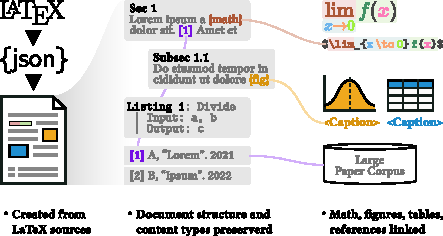
\includegraphics[width=\linewidth]{figures/ref_covgran/schema}
  % \caption{Schematic of our data set.\\
  %   \footnotesize\normalfont Created from arXiv.org \LaTeX\ sources, our data set preserves document \emph{sctructure} (sections, subsections, ...) and \emph{content types} (paragraphs, listings, ...). In-text positions of mathematical notation, figures, tables and citation markers are linked to \LaTeX\ math content, figure/table captions, and bibliographic references respectively. Bibliographical references are linked to the large paper corpus OpenAlex.
  % }
  \caption[Schematic of our data set]{Schematic of our data set. (Created from arXiv.org \LaTeX\ sources, our data set preserves document sctructure (sections, subsections, ...) and content types (paragraphs, listings, ...). In-text positions of mathematical notation, figures, tables and citation markers are linked to \LaTeX\ math content, figure/table captions, and bibliographic references respectively. Bibliographical references are linked to the large paper corpus OpenAlex.}
  \label{fig:schema}
\end{figure}

% - - - - - What are key shortcomings of current data sets? (research gap)

Key aspects of such data sets are (1)~basic measures such as quality, size, and temporal as well as disciplinary coverage, (2)~their citation network, and (3)~handling of non-textual content. (1)~Quality is affected by the source material (e.g. PDF or \LaTeX) and parsing method. (2)~The citation network is important to allow for bibliometric analyses. (3)~Non-textual content such as tables, figures, and mathematical notation often contain important information.

Across these key aspects, we see significant shortcomings in currently available data sets, as shown in Table~\ref{tab:comparison}. For example, (1)~limited size (SciXGen), (2)~omission of a citation network (arXMLiv), and (3)~no or limited handling of mathematical notation (S2ORC, unarXive 2020).

% NOTES
%
% S2ORC (PDF) math
% - convert to unicode -> error-prone & limited
%
% SciXGen
% - focus on text generation
% - demo domain expired, undocumented data on GitHub
% - https://aclanthology.org/2021.findings-emnlp.128/
% - https://github.com/sairin1202/SciXGen
%
%
% PMC OAS
% get file list CSVs from here: https://ftp.ncbi.nlm.nih.gov/pub/pmc/oa_bulk/oa_comm/xml/
% $ ls oa_comm_xml.PMC00*xxxxxx.baseline.2023-02-08.filelist.csv
%    oa_comm_xml.PMC000xxxxxx.baseline.2023-02-08.filelist.csv
%    oa_comm_xml.PMC001xxxxxx.baseline.2023-02-08.filelist.csv
%    oa_comm_xml.PMC002xxxxxx.baseline.2023-02-08.filelist.csv
%    oa_comm_xml.PMC003xxxxxx.baseline.2023-02-08.filelist.csv
%    oa_comm_xml.PMC004xxxxxx.baseline.2023-02-08.filelist.csv
%    oa_comm_xml.PMC005xxxxxx.baseline.2023-02-08.filelist.csv
%    oa_comm_xml.PMC006xxxxxx.baseline.2023-02-08.filelist.csv
%    oa_comm_xml.PMC007xxxxxx.baseline.2023-02-08.filelist.csv
%    oa_comm_xml.PMC008xxxxxx.baseline.2023-02-08.filelist.csv
%    oa_comm_xml.PMC009xxxxxx.baseline.2023-02-08.filelist.csv
% $ cat oa_comm_xml.PMC00*xxxxxx.baseline.2023-02-08.filelist.csv | wc -l
%    3296051

% - - - - - How is this research gap closed? (conceptional) - - - - -

To address these issues, we propose a new version of the data set unarXive, %\footnote{The \LaTeX\ based data set for NLP on Academic Text}
which comprises 1.9 M publication across several disciplines, includes a more complete citation network than its predecessors, and retains structured mathematical notation as well as table and figure captions (see Figure~\ref{fig:schema}).  % captions = “textual surrogates”
Apart from the data set itself, we furthermore provide ready-to-use training and test data for two NLP tasks. Overall, we make the following contributions.

% - - - - - List of contributions, shared data, etc. (name numbers, facts, links to data, etc.) - - - - -

\begin{itemize}
    \item We provide a 1.9 M document scholarly data set, containing structured full-text, annotated in-text citations, linked table and figure captions, structured mathematical notation, and a hight quality citation network.
    \item We provide ready-to-use training/test data for the development and evaluation of approaches to two NLP tasks, namely citation recommendation and IMRaD classification.
    \item We distribute our data in accordance to the FAIR principles~\cite{Wilkinson2016} and share our source code freely available under a permissive license.
\end{itemize}

\afterpage{  % - - - start of afterpage
\begin{landscape}
\begin{table}
  % \caption{
  %   Comparison of large data sets derived from paper full-texts\\
  %   {\footnotesize\normalfont
  %    $^\dagger$Cit. network completeness is reported is two ways. ``general'': the whole data set; not directly comparable. ``compare'': for arXiv.org data from 1991--2020; directly comparable.\\
  %    $^\ddagger$References in the PMC OAS are partially linked to a mixed set of IDs (PubMed, MEDLINE, DOI)~\cite{Gipp2015}. Therefore there is no single, comprehensive number for its completeness.
  %   }
  %  }
  \caption[Comparison of large data sets derived from paper full-texts]{Comparison of large data sets derived from paper full-texts ($^\dagger$Cit. network completeness is reported is two ways. ``general'': the whole data set; not directly comparable. ``compare'': for arXiv.org data from 1991--2020; directly comparable. $^\ddagger$References in the PMC OAS are partially linked to a mixed set of IDs (PubMed, MEDLINE, DOI)~\cite{Gipp2015}. Therefore there is no single, comprehensive number for its completeness.}
  \label{tab:comparison}
  \begin{tabular}{lccccccccc}
    \toprule
    \ & \multicolumn{2}{c}{Source} & \multicolumn{2}{c}{\hphantom{wi}Citation Network$^\dagger$} & \multicolumn{2}{c}{Structured} & \ & \ & \ \\
    Data Set & Data & Format & general & compare & Doc. & Math. & \# Docs & Disciplines & Purpose \\
    \midrule
    CORE~\cite{core} & multiple & PDF & 0\% & - & $\times$ & $\times$ & $>$100 M & various & general NLP \\
    S2ORC (PDF)~\cite{Lo2020} & multiple & PDF & 69.4\% & - & \checkmark & $\times$ & 12 M & various & general NLP \\
    % (19.3+6.8)/(27.8+21.9) = 53% overall, 69.4% GROBID parses, 31.1% LaTeX parses
    unarXive 2020~\cite{Saier2020} & arXiv.org & \LaTeX & 42.6\% & 42.6\% & $\times$ & $\times$ & 1.2 M & phys., maths, CS & general NLP \\
    \midrule
    S2ORC (\LaTeX)~\cite{Lo2020} & arXiv.org & \LaTeX & 31.1\% & 31.1\% & \checkmark & \checkmark & 1.5 M & phys., maths, CS & general NLP \\
    arXMLiv~\cite{arXMLiv} & arXiv.org & \LaTeX & 0\% & 0\% & \checkmark & \checkmark & 1.6 M & phys., maths, CS & maths linguistics \\
    SciXGen~\cite{chen2021-scixgen} & arXiv.org & \LaTeX & 41.6\% & - & \checkmark & \checkmark & 205 k & CS & text generation \\
    PMC OAS\textsuperscript{14} & PubMed & XML & mixed$^\ddagger$ & - & \checkmark & \checkmark & \textbf{3.3 M} & \textbf{biomedical} & not NLP specific \\  % TODO: make sure this footnotemark still is correct in the end, or convert the table to a threeparttable with its own tablenotes
    \textbf{unarXive 2022} (ours) & arXiv.org & \LaTeX & 44.4\% & \textbf{44.4\%} & \textbf{\checkmark} & \textbf{\checkmark} & \textbf{1.9 M} & \textbf{phys., maths, CS} & general NLP \\
    % 0.4441 for 1991—2022, 0.4438 for 1991–2020
    \bottomrule
  \end{tabular}
\end{table}
\end{landscape}
}  % - - - end of afterpage

\subsection{Related Work}

In Table~\ref{tab:comparison} we give an overview of related work.
Excluded are data sets that are either just sets of PDFs, or only contain metadata.

CORE~\cite{core}, while being very large, does not contain a citation network, nor is document structure preserved.
S2ORC (PDF)~\cite{Lo2020} is second in size and, while not directly comparable due to different publications covered, has the most complete citation network. However, mathematical notation is only partially preserved as plaintext.
unarXive 2020~\cite{Saier2020} has the second highest citation network completeness in direct comparison, but lacks structured content.

The bottom part of the table are data sets with both document structure preserved and structured mathematical notation.
S2ORC (\LaTeX)~\cite{Lo2020} is a discontinued\footnote{Last release including the \LaTeX\ subset is 2019-09-28, see \refurlinline{https://github.com/allenai/s2orc}{2023-02-12}.} subset of S2ORC and has a limited citation network, 
arXMLiv~\cite{arXMLiv} offers the highest level of structure but no citation network, and 
SciXGen~\cite{chen2021-scixgen} is limited in size.
The PMC OAS\refurl{https://www.ncbi.nlm.nih.gov/pmc/tools/openftlist/}{2023-11-06} is comparable to unarXive 2022 in size and structure, but has a partial and mixed citation network.


Overall, unarXive 2022 has the most complete citation network as far as direct comparison is possible, preserves document structure as well as structured mathematical notation, and is the largest data set covering physics, mathematics and computer science.

\subsection{Approach}
% How the data sets was created

We base our data set creation approach in part on S2ORC (\LaTeX) and in part on unarXive 2020. This is motivated as follows.

As shown in Table~\ref{tab:comparison}, the majority of related data sets is based on paper's \LaTeX\ sources---which is less noise-prone than parsing PDFs~\cite{Bast2017}. Among these, S2ORC (\LaTeX) provides well structured full-text content usable for a wide variety of applications (see Section~\ref{sec:applications}), while arXMLiv and SciXGen are optimized for special purposes. We therefore base our structured document representation on S2ORC (\LaTeX). Regarding the citation network, however, unarXive 2020 achieves the most high-quality results in direct comparison among existing data sets. We therefore base our citation network creation on unarXive 2020.

Regarding both S2ORC (\LaTeX) and unarXive 2020, we do not just copy, but also improve upon the existing work. To furthermore provide an up-to-date data set, we use as source data all papers on arXiv.org up until the end of 2022.

Conceptually, our overall data set creation process can be broken down into two major steps, namely document parsing and reference linking, In the following these are described in more detail.

\subsubsection{Document Parsing}
To convert the \LaTeX\ source of a paper into a format that is well suited for NLP applications and analyses, we follow S2ORC (\LaTeX) and unarXive 2020 and perform the following three steps. First, we flatten the paper's \LaTeX\ source into a single \texttt{.tex} document using latexpand.\refurl{https://ctan.org/pkg/latexpand}{2023-11-10} Next, we use the tool Tralics\refurl{https://www-sop.inria.fr/marelle/tralics/}{2023-11-10} to convert the \LaTeX\ source into XML. In the last step, we create an easy to handle JSON structure from the XML.

We adapt and extend the JSON structure of S2ORC as shown in Table~\ref{tab:formext}. Adding paper metadata facilitates easier analyses (e.g. for specific or across disciplines). Including information on section numbers and types reflects the document structure more closely (e.g. the nesting structure is not lost). Retaining URLs from embedded links helps with reference linking (see Section~\ref{sec:reflink}).

We mark the position of citation markers, tables, figures, and mathematical notation within the running text, and link citations markers to their references, tables and figures to their captions (i.e., textual surrogates of their content), and mathematical notation to its original \LaTeX\ content.

\begin{table}
  \centering
  \caption{Extension of S2ORC format}
  \label{tab:formext}
  \begin{tabular}{p{2cm}p{5cm}p{6.5cm}}
    \toprule
    Entity & S2ORC data & Added data \\
    \midrule
    \textbf{Paper} &
        \begin{minipage}[t]{\linewidth}
            \begin{itemize}[nosep,after=\strut,leftmargin=1mm]
                \item ID
                \item abstract
                \item full-text (list of paragraphs)
                \item bibliographic references
            \end{itemize}
        \end{minipage} &
        \begin{minipage}[t]{\linewidth}
            \begin{itemize}[leftmargin=1mm]
                \item Metadata (title, list of authors, discipline, license, version history)
            \end{itemize}
        \end{minipage}\\
    %\midrule
    \textbf{Paragraph} &
        \begin{minipage}[t]{\linewidth}
            \begin{itemize}[leftmargin=1mm]
                \item Section title 
                \item text
            \end{itemize}
        \end{minipage} &
        \begin{minipage}[t]{\linewidth}
            \begin{itemize}[leftmargin=1mm]
                \item Section number 
                \item Section type (e.g. \textit{section}, \textit{subsection}) 
                \item Content type (e.g. \textit{paragraph}, \textit{listing}, \textit{proof})
            \end{itemize}
        \end{minipage}\\
    %\midrule
    \textbf{Bib\-li\-o\-gra\-phic reference} &
        \begin{minipage}[t]{\linewidth}
            \begin{itemize}[leftmargin=1mm]
                \item Parsed reference
                \item ID of cited document
            \end{itemize}
        \end{minipage} &
        \begin{minipage}[t]{\linewidth}
            \begin{itemize}[leftmargin=1mm]
                \item Raw reference string
                \item List of contained arXiv IDs
                \item List of embedded links (i.e., URLs of clickable links not rendered as text when viewing the document)
            \end{itemize}
        \end{minipage}\\
  \bottomrule
\end{tabular}
\end{table}

\subsubsection{Reference Linking}\label{sec:reflink}

To add a citation network to the data set, bibliographical references---which at this point are just raw strings of text---need to be associated with the cited documents they are referencing. We follow the methodology of unarXive 2020 and link references to a large corpus of publication metadata. To do this, references are first parsed to determine the contained information (title, authors, year, venue, etc.), which is then matched against the paper records in the large metadata corpus. For these two steps, we make the following changes and improvements to the unarXive 2020 approach.

\paragraph{Parsing} unarXive 2020 utilizes the tool Neural Parscit~\cite{neuralparscit} for reference parsing and furthermore uses a heuristic procedure to determine identifiers such as DOIs or arXiv IDs found within reference string. We use GROBID~\cite{Lopez2009}, a more commonly used and actively developed tool. Additionally, we extend the identifier determination heuristics to be more robust and versatile by refining matching patterns and extending them to more citation styles.

\paragraph{Matching} unarXive 2020 matches references to paper records in the Microsoft Academic Graph (MAG)~\cite{Sinha2015}, which is no longer publicly available. Instead of the MAG, we use OpenAlex~\cite{openalex}, the MAG's open successor provided by the nonprofit organization OurResearch.\refurl{https://ourresearch.org/}{2023-11-10} Chosing OpenAlex allows us to also match references to recent papers, which would not be contained in legacy versions of the MAG. Additionally, the fact that OpenAlex paper records contain a variety of identifiers (e.g. DOI and PubMed ID) facilitates combined and comparative analyses of our data with others. Furthermore, OpenAlex has been deemed better suited for bibliographic analyses than the MAG~\cite{openalex-vs-mag}.

% if we need scientific foundation for the decision to choose OpenAlex:
% a recent research comparing MAG's and OpenAlex suitability for bibliometric work concludes: " OpenAlex seems to be more suited for bibliometric analyses than MAG"
% see: https://arxiv.org/abs/2206.14168 

% OpenAlex contains metadata on scholarly documents and related entities, such as authors and institutions. Regular (biweekly) updates, extensive coverage (of more than 247 million documents) and an emphasis on standardized document identifiers (, specifically DOI, PubMed ID and PMC ID,) make the use of OpenAlex for our reference matching promising~\cite{openalex}.

% OurResearch website: https://ourresearch.org/ (in footnote?)
% today: 247,826,959 documents in OpenAlex. Retrieved through API call: https://api.openalex.org/works 
% DOI rate: 143,111,972 of all docs have DOI maintained = 57\.8%
% for recent years much higher: 2020 : 0.74, 2021 : 0.86, 2022 : 0.98 (higher than in MAG)

\subsection{Results}

In the following, we first present key statistics of our proposed data set. Following that, we explain how the data set can be used for analyses as well as the development of NLP applications, and introduce training/test data for two NLP tasks. Lastly, we describe how the data set is distributed to facilitate easy adoption by the community of researchers and practitioners.

\subsubsection{Data Set}

% Stats and figures, exemplary findings/interesting obsevations as

Our data set comprises \emph{1,881,346 papers}, which contain a combined \emph{182,586,547} paragraphs, \emph{63,367,836 references} and \emph{133,744,613 in-text citation markers}. The distribution across disciplines is 57\% physics, 20\% mathematics, 17\% computer science, and a combined 5\% for others. %statistics, electrical engineering and systems science, quantitative biology, quantitative finance, and economics.
We are able to link 28,135,565 references (44.4\%) and 64,547,944 (48.3\%) in-text citation markers to OpenAlex. As shown in Table~\ref{tab:comparison}, this makes our citation network more complete than that of existing data sets.

In Listing~\ref{lst:datasample} we show an excerpt of our document representation for one paper, showcasing the extracted plain text and structured content.

\begin{lstlisting}[language=json,caption=Data example.,label=lst:datasample,breaklines=true,captionpos=b,frame=single,showlines=true,basicstyle=\tiny]
/* - - - - - - - example paper (arXiv:2105.05862) - - - - - - - */
{ "paper_id": "2105.05862",
  "metadata": {...},
  "abstract": {...},
  "body_text": [...],
  "ref_entries": {...},
  "bib_entries": {...} }
/* - - - - - - - one of the sections in body_text - - - - - - - */
{ "section": "Memory wave form",
  "sec_number": "2.1",
  "sec_type": "subsection",
  "content_type": "paragraph",
  "text": "The gauge choice leading us to this solution does not fix
           completely all the gauge freedom and an additional constraint
           should be imposed to leave only the physical degrees of freedom.
           This is done by projecting the source tensor {{formula:7fd88bcd-
           9013-433d-9756-b874472530d9}} into its transverse-traceless (TT)
           components (see for example {{cite:80dbb6c8b9c12f561a8e585faceac5f
           4e104d60d}}). Doing this and without loss of generality, we will
           use the following very well known ansatz for the source term
           proposed in {{cite:bc9a8ca19785627a087ae0c01abe155c22388e16}}\n" }
/* - - - - - - - ref_entries entry for {{formula:7fd88...}} - - - - - - - */
{ "latex": "S_{\\mu \\nu }",
  "type": "formula" }
/* - - - - - - - bib_entries entry for {{cite:80dbb...}} - - - - - - - */
{ "bib_entry_raw": "R. Epstein, The Generation of Gravitational Radiation by Esc
                    aping Supernova Neutrinos, Astrophys. J. 223 (1978) 1037.",
  "contained_links": [
    { "url": "https://doi.org/10.1086/156337",
      "text": "Astrophys. J. 223 (1978) 1037.",
      "start": 87,
      "end": 117 }
  ],
  "ids" {...} }
\end{lstlisting}

In Figure~\ref{fig:numpprs} we show the number of papers across all disciplines over all years covered. We can see that yearly arXiv.org submissions in computer science are likely to surpass those in physics in 2023. As a simple showcase of the use of structured full-text content, we show in Figure~\ref{fig:refdensity} how the average number of bibliographic references per paragraph developed over time for the three major disciplines represented in the data set. Dividing by paragraphs is done to account for variation in paper length. We can see that the density of references is increasing more rapidly in physics and computer science, than it is in mathematics.

\begin{figure}
  \centering
  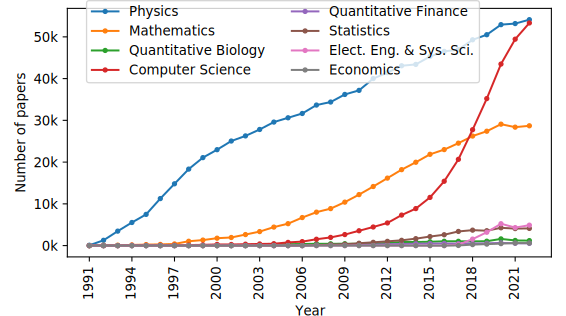
\includegraphics[width=0.7\linewidth]{figures/ref_covgran/numpprs}
  \caption{Number of papers per year.}
  \label{fig:numpprs}
% \end{figure}

% \begin{figure}
%   \centering
  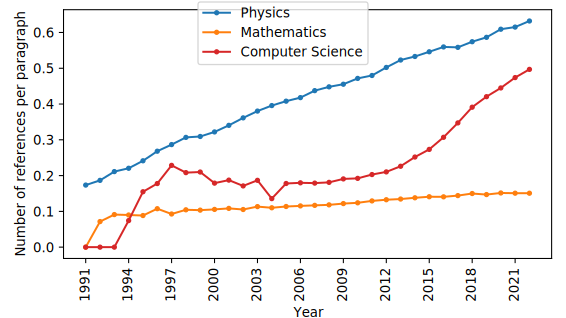
\includegraphics[width=0.7\linewidth]{figures/ref_covgran/refdensity}
  \caption{Reference density per year.}
  \label{fig:refdensity}
\end{figure}

% Physics: 1080760
% Mathematics: 380362
% Quantitative Biology: 16638
% Computer Science: 327207
% Quantitative Finance: 7933
% Statistics: 36717
% Electrical Engineering and Systems Science: 28212
% Economics: 3517

\subsubsection{Applications}\label{sec:applications}
% Applications and concrete examples how the research community benefits
% from this data set and what has been done to facilitate this

% \item Application cases/tasks
% \begin{itemize}
%     \item Citation recommendation
%     \item IMRaD classification
%     \item ...
% \end{itemize}

As is evident by the past use of our data set's predecessors unarXive 2020 and S2ORC, large-scale scholarly data sets created with NLP research in mind have broad applicability. Example uses are analyses of citation behavior across languages~\cite{Saier2021} or disciplines~\cite{Veneri2022} and the development of models for claim verification~\cite{wadden2020}, document retrieval~\cite{Parisot2022}, summarization~\cite{citesum}, or information extraction~\cite{viswanathan2021}.

Due to its similarities in structure and contained information, unarXive 2022 is equally suitable for the applications named above. Beyond these, we provide data for two NLP tasks on unarXive 2022, namely content based citation recommendation and IMRaD classification, which are described in the following.

\paragraph{Content Based Citation Recommendation}
Given a piece of text and a citation-marker position, the task of content based citation recommendation entails identifying publications which are suitable to cite in the given text at the given position~\cite{Bhagavatula2018,Faerber2020a}. Large full-text corpora of publications with a citation network provide a rich source for supervision of machine learning (ML) models for this task. That is, human made citations are used as training examples, or for evaluating models in a citation re-prediction setting.
From the premissively licensed papers in our data set we use all in-text citation markers with a linked reference cited at least three times, to allow splitting into train, dev, and test data.
The result is 2.5 M items consisting of (1) a paragraph and citation marker position (model input), and (2) the ID of the cited document (desired model output). % maybe add some stats on # of cited docs, etc.
% The data is available at \refurlinline{https://huggingface.co/datasets/saier/unarXive_citrec}.

\paragraph{IMRaD Classification}
Scientific publications are usually structured into sections commonly summarized as ``Introduction, Methods, Results, and Discussion'' (IMRaD). Classifying sections of scientific text into these four classes is done, for example, in fine-grained citation classification. % ---to answer, for example, if a publication was cited as background information in the introduction, or as an influence on the methodology in the methods section.
Because conventions differ between disciplines, we prepare data for this task for computer science papers only. To aforementioned four classes we add the common ``Related Work'' section as a fifth class. From the premissively licensed computer science papers in our data, we use those that are unambiguously assignable to one of the five classes. The result is 530~k items consisting of (1) the paragraph text (model input), and (2) the class (desired model output). An exemplary application scenario for a model trained on this data is a paper writing assistant that can detect parts in a manuscript, which might be better placed in a different section (e.g. discussion rather than results).
% The data is available at \refurlinline{https://huggingface.co/datasets/saier/unarXive_imrad_clf}{2023-11-10}.


% 277388 CS papers
% 1604694 non CS papers
% defaultdict(<class 'int'>,
%             {'discussion': 555271,
%              'introduction': 1826742,
%              'methods': 424280,
%              'other': 19323579,
%              'related_work': 385052,
%              'results': 273471})
% 3464816 IMRaDR papras

\subsubsection{Distribution}

% - Zenodo
% - Permissively licenced subset
%     - CC: 197315
%     - public domain: 9779
%     -> 207094
%     207094/1881346 = 11.0078 %
% - Huggingface dataloader

Under consideration of the FAIR principles, we chose the following well established distribution channels and licenses for our data set, aforementioned NLP task data, as well as our source code.

\begin{itemize}
    \item The \textbf{data set} is distributed on \texttt{Zenodo}.\\
        \begin{small}
        $\rightarrow$\refurlinline{https://doi.org/10.5281/zenodo.7752615}{2023-11-10} (open subset)\\
        $\rightarrow$\refurlinline{https://doi.org/10.5281/zenodo.7752754}{2023-11-10} (full)\\
        \end{small}
        In accordance with the licensing terms of our source data, we share our data set in two versions.\\
        (1) The subset generated from permissively licensed source data (165 k publications, 9\%) is openly accessible.\\
        (2) The full data set, generated partially from source data under arXiv.org's ``non-exclusive license to distribute,''\refurl{http://arxiv.org/licenses/nonexclusive-distrib/1.0/}{2023-11-10} is accessible through Zenodo's ``restricted access'' policy,\refurl{https://about.zenodo.org/policies/}{2023-11-10}
making it possible to grant access to the data on request given the intended use is in accordance with the license terms.
    \item The \textbf{NLP task data} is provided on the \texttt{Hugging Face Hub}.\\
        \begin{small}
        $\rightarrow$\refurlinline{https://hf.co/datasets/saier/unarXive_citrec}{2023-11-10}\\
        $\rightarrow$\refurlinline{https://hf.co/datasets/saier/unarXive_imrad_clf}{2023-11-10}\\
        \end{small}
        This facilitates easy access and use by the NLP community.
    \item The \textbf{source code} for creating the data set is shared on \texttt{GitHub} under the MIT License.\\
        \begin{small}
        $\rightarrow$\refurlinline{https://github.com/IllDepence/unarXive}{2023-11-10}\\
        \end{small}
        Sharing the code openly and permissively licensed allows anyone to freely modify and extend the code to their needs. This makes, for example, integration into other NLP projects such as benchmarks and frameworks possible.
\end{itemize}

\subsection{Conclusion}
We propose unarXive 2022, a data set generated from 1.9 M \LaTeX\ paper sources and suitable for a wide variety of analyses and NLP applications. We base our approach to data set creation and format on existing works, while also addressing their shortcomings. Improving upon these tried and tested predecessors, unarXive 2022 offers the most complete citation network and most structured content compared to existing data sets, and is surpassed in size only by the PMC OAS, which covers a different set of disciplines.

With our data set we provide data for two NLP tasks, content based citation recommendation and IMRaD classification, to facilitate its usage. We furthermore distribute our work under consideration of the FAIR principles, sharing it through well established channels and permissively licensed, thereby ensuring proper accessibility, easy use, and possibilities for adaption and extension.

We plan to incrementally update our data set with new arXiv.org submissions. For future developments, we note the importance of mathematical notation in academic publications, as reflected by recent SemEval tasks in 2021 and 2022~\cite{semeval21_task8,semeval22_task12}. Similar to existing projects,\refurl{https://github.com/PierreSenellart/theoremkb}{2023-11-10} we plan to investigate novel analyses and applications based on the combination of our data set's citation network and structured mathematical notation.

% Possible addition: \cite{Meuschke2023} -> PDF extraction still struggles w/ mathematical notation across the board, so mathematical notation is not only important but also hard to get by

% Publications in many scientific disciplines communicate key information through numbers and formulae. Accordingly, the extraction of such information has recently gained attention~\cite{semeval21_task8,semeval22_task12}

% In [10]: np.sum(mtrs['num_para_type_proof'])
% Out[10]: 2014983.0

% \cite{delemazure2020}

\subsection{Author Contributions}  % cf. https://credit.niso.org/
Tarek Saier: Conceptualization, Data curation (lead), Formal analysis, Methodology, Software (lead), Visualization, Writing -- original draft, Writing -- review \& editing. Johan Krause: Data curation (support), Software (support). Michael F{\"a}rber: Writing -- review \& editing.

%%
%% The acknowledgments section is defined using the "acks" environment
%% (and NOT an unnumbered section). This ensures the proper
%% identification of the section in the article metadata, and the
%% consistent spelling of the heading.
\subsection{Acknowledgements}
This work was partially supported by the German Federal Ministry of Education and Research (BMBF) via [KOM,BI], a Software Campus project (01IS17042).
The authors acknowledge support by the state of Baden-W{\"u}rttemberg through bwHPC.
We thank Johannes Reber for supporting early stages of the software development.

\section{Result Assessment}
\label{sec:covgran-assessment}

The work in this chapter addresses the following research task.

\begin{rtlist}
    \item[\rtmark{2}:] \textit{Citation Network Completeness} - develop a method to link literature references, that is able to link more references than are linked in existing data sets, while not compromising on link correctness or processing efficiency.
\end{rtlist}

With the inter-reference blocking and matching method presented in Section~\ref{sec:covgran-blocking} we achieve a 90\% increase in linked references, a five-fold increase in bibliographic couplings, and a nine-fold increase in connected in-text citation markers.
Furthermore, with the improved corpus creation method presented in Section~\ref{sec:covgran-ux22}, we achieve a new state-of-the-art reference matching success rate of 44.4\%. Different from our contributions to \rtmark{2} in Chapter~\ref{chp:corpus}, we are here able to make direct comparisons to related work. Our reference matching success rate of 44.4\% compares favorably to our previously method (42.6\%), S2ORC (31.1\%), and arXMLiv (no citation network). Accordingly, we deem \rtmark{2} successfully achieved.

In terms of the overarching research goal of enabling higher-quality scholarly data (see Table~\ref{tab:scholdataquali} in Chapter~\ref{chp:foundations}), the work presented in this chapter makes the following contributions.

\begin{infobox-progress}
      \textbf{Scholarly Data Quality Contributions - \cite{Saier2022ULITE,Saier2023unarXive}}\vspace{0.5em}

      \begin{tabular}{lp{10.9cm}}
        \toprule
        Crit. & Contribution \\
        \midrule
        $\mathbf{Rel_{SDR}}$ & Mathematical notation included in the structured document representation \\
        $\mathbf{Tim_{C/S}}$ & Publications included up until end of the most recent full year \\
        $\mathbf{Coy_{CN}}$ & OpenAlex, arXiv, and PubMed IDs as well as DOIs included \\
        $\mathbf{Coy_{SDR}}$ & Section structure and section type information included \\
        $\mathbf{Cos_{CN}}$ & Blocking and matching procedure enabling increase linked references and bibliographic couplings \\
        $\mathbf{Cos_{SDR}}$ & Full-text of documents as well as figure and table captions included \\
        \bottomrule
      \end{tabular}
\end{infobox-progress}

$\mathbf{Rel_{SDR}}$ Our improved document conversion methodology provides structured mathematical notation as part of our document representations. The resulting data is therefore of high relevance for use cases focussing on phenomena manifested within them, such as mathematical information retrieval~\cite{semeval22_task12} and the analysis of theorems\refurl{https://github.com/PierreSenellart/theoremkb}{2024-02-04}. Our data source being arXiv, which has a large coverage of physics, mathematics, and computer science papers, additionally is beneficial in this regard, as all three are disciplines, where mathematical notation is comparably relevant and frequently used.

$\mathbf{Tim_{C/S}}$ We apply our method for generating scholarly data on all documents on arXiv until end of the most recent full year. Accordingly, the resulting corpus contains more recent documents than data sets released earlier.

$\mathbf{Coy_{CN}}$ By linking references to OpenAlex, we are able to provide a large number of document identifiers in our citation network. In particular these are OpenAlex IDs, arXiv IDs, PubMed IDs, and DOIs. This makes our data a versatile target for comparing and combining it with other data.

$\mathbf{Coy_{SDR}}$ Our document representation provides a section and paragraph structure as well as paragraph type information (text, listing, etc.). This enables fine-grained document content comparison, filtering, and combination with external data. % TODO: comparison to other datasets (S2ORC, arXMLiv, PMC OAS)

$\mathbf{Cos_{CN}}$ With our inter-reference blocking and matching method, we provide a means to improve citation network completeness through increased linked references (Section~\ref{sec:covgran-blocking}). Furthermore, our improved corpus creation method achieves a new state-of-the-art reference matching success rate of 44.4\% (Section~\ref{sec:covgran-ux22})

$\mathbf{Cos_{SDR}}$ In addition to papers' full-text content, we provide figure and table captions linked within the text. This makes our structured document representations more complete than before.
